\documentclass[12pt,letterpaper]{article}

\usepackage[utf8]{inputenc}
\usepackage[english]{babel}
\usepackage{amsmath}
\usepackage{amsthm}
\usepackage[left=2cm,right=2cm,top=2cm,bottom=2cm]{geometry}
\usepackage{color}
\usepackage{mathtools}
\usepackage{amssymb}
\usepackage{setspace}
\usepackage{fullpage}
\usepackage{times}
\usepackage{color}
\usepackage{hyperref}
\usepackage{url}
\usepackage{enumerate}
\usepackage{graphicx}
\usepackage{bm}
\usepackage{tcolorbox}
\usepackage[parfill]{parskip}
\usepackage{listings}
\usepackage{bbm}
\usepackage{tikz}
\usetikzlibrary{automata}
\usetikzlibrary{fit}
\usetikzlibrary{positioning}
\usetikzlibrary{arrows}
\usetikzlibrary{backgrounds}



 \definecolor{codegreen}{rgb}{0,0.6,0}
    \definecolor{codegray}{rgb}{0.5,0.5,0.5}
    \definecolor{codepurple}{HTML}{C42043}
    \definecolor{backcolour}{HTML}{F2F2F2}
    \definecolor{bookColor}{cmyk}{0,0,0,0.90}  
    \color{bookColor}

    \lstset{upquote=true}

    \lstdefinestyle{mystyle}{
        backgroundcolor=\color{backcolour},   
        commentstyle=\color{codegreen},
        keywordstyle=\color{codepurple},
        stringstyle=\color{codepurple},
        basicstyle=\small,
        breakatwhitespace=false,         
        breaklines=true,                 
        captionpos=b,                    
        keepspaces=true,                 
        numbersep=-10pt,                  
        showspaces=false,                
        showstringspaces=false,
        showtabs=false,      
    }
    \lstset{style=mystyle}

\title{LeetCode Technical Writing \vspace{-20pt}}
\author{Hoon Oh}
%\date{\vspace{-15pt} April 16, 2018\vspace{-15pt}}


\newtheorem{theorem}{Theorem}
\newtheorem{problem}{Problem}
\newtheorem{lemma}{Lemma}
\newtheorem{question}{Question}
\newtheorem{definition}{Definition}
\newtheorem{example}{Example}
\newcommand{\C}{\mathcal{C}}
\newcommand{\N}{\mathbb{N}}
\newcommand{\E}{\mathbb{E}}
\newcommand{\R}{\mathbb{R}}
\newcommand{\Q}{\mathbb{Q}}
\renewcommand{\P}{\mathcal{P}}
\renewcommand{\dim}{\mathrm{dim}}
\newcommand{\range}{\mathcal{range}}
\newcommand{\Astar}{$\mathrm{A^*}~$}
\newcommand{\cost}{\mathrm{c}}
\newcommand{\mms}{\mathrm{MMS}}
\newcommand{\red}[1]{{\color{red} #1}}

\DeclareMathOperator*{\minimize}{minimize}
\DeclareMathOperator*{\maximize}{maximize}
\DeclareMathOperator*{\diag}{diag}
\DeclareMathOperator*{\subjectto}{subject\;to}
\DeclareMathOperator*{\vect}{vec}

\newcommand{\lp}[0]{\left (}
\newcommand{\rp}[0]{\right )}
\newcommand{\F}{\mathcal{F}}
\newcommand{\OPT}{\mathrm{OPT}}

\newcommand{\fs}{\mathfrak{s}}
\newcommand{\ft}{\mathfrak{t}}
\newcommand{\fv}{\mathfrak{v}}

\renewcommand{\vec}[1]{\boldsymbol{\mathbf{#1}}}


\DeclareMathOperator{\sign}{sign}
\DeclareMathOperator{\tr}{tr}
\newcommand{\Value}[1]{\operatorname{value}(#1)}

\newcommand{\edges}{\mathtt{edges}}
\newcommand{\from}{\mathtt{from}}
\newcommand{\too}{\mathtt{to}}

\begin{document}

\maketitle



\section*{1557. Minimum Number of Vertices to Reach All Nodes [Medium]}
\begin{tcolorbox}
Given a \textbf{directed acyclic graph}, with $n$ vertices numbered from $0$ to $n-1$,
 and an array $\edges$ where $\edges[i] = [\from_i, \too_i]$ represents a directed edge from node $\from_i$ to node $\too_i$.

\vspace{5pt}

Find \textit{the smallest set of vertices from which all nodes in the graph are reachable}. It's guaranteed that a unique solution exists.
\vspace{5pt}

Notice that you can return the vertices in any order.

\end{tcolorbox}

\section{ An Example}

\begin{figure}[h]
\centering
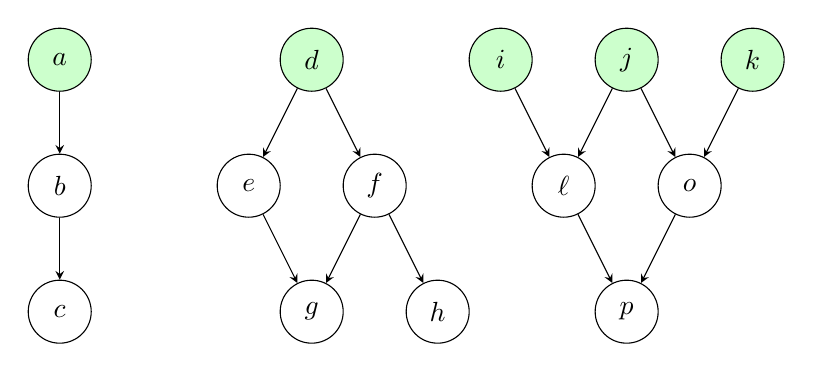
\begin{tikzpicture}[scale=0.8,
		main/.style={shape=circle, draw=black,minimum size= 0.8cm},
]

\node[main,fill=green!20] (a) at (0,6) {$a$};
\node[main] (b) at (0,4) {$b$};
\node[main] (c) at (0,2) {$c$};

\node[main,fill=green!20] (d) at (4,6) {$d$};
\node[main] (e) at (3,4) {$e$};
\node[main] (f) at (5,4) {$f$};
\node[main] (g) at (4,2) {$g$};
\node[main] (h) at (6,2) {$h$};


\node[main,fill=green!20] (i) at (7,6) {$i$};
\node[main,fill=green!20] (j) at (9,6) {$j$};
\node[main,fill=green!20] (k) at (11,6) {$k$};
\node[main] (l) at (8,4) {$\ell$};
\node[main] (o) at (10,4) {$o$};
\node[main] (p) at (9,2) {$p$};


\draw [->, >=stealth] (a) -- (b);
\draw [->, >=stealth] (b) -- (c);
\draw [->, >=stealth] (d) -- (e);
\draw [->, >=stealth] (e) -- (g);
\draw [->, >=stealth] (d) -- (f);
\draw [->, >=stealth] (f) -- (g);
\draw [->, >=stealth] (f) -- (h);
\draw [->, >=stealth] (i) -- (l);
\draw [->, >=stealth] (j) -- (l);
\draw [->, >=stealth] (j) -- (o);
\draw [->, >=stealth] (k) -- (o);
\draw [->, >=stealth] (l) -- (p);
\draw [->, >=stealth] (o) -- (p);


\end{tikzpicture}
\caption{An instance of directed acyclic graph.The smallest set of vertices from which all nodes in the graph are reachable is the set $\{a,d,i,j,k\}$.}
\label{fig:ex}
\end{figure}



\section{A variant of Union-find Method}

\paragraph{Intuition}

We can view the problem as a variant of union-find problem. If a node $u$ is reachable from a node $v$ then we want to group $u$ and $v$ together.
However in Figure \ref{fig:ex}, we do not want to group nodes $i$ and $j$ in the same group. 
We resolve this problem by combining $u$ and $v$ to the same group only if there is an edge from $u$ to $v$ and $v$ does not belong to another group.

\paragraph{Algorithm}
We initialize each node's group head as itself. In other words, a node $u$'s group head is $u$.
We go through each directed edge $(u,v)$ (edge from $u$ to $v$). If $v$'s group head is itself, then label $v$'s group with $u$'s group head.
Then at the end of the algorithm, output the set of distinct group heads as our solution.  

At any time of the algorithm, a node $v$ can be reached by the node correspond to $v$'s group head.
This is true because either the group head is $v$'s parent, or a it is node that can reach the parent.
Furthermore, at the end of the algorithm there is no group head $u$ that can reach another group head $v$.
This is true because if such path exists, then there must exists an edge to $v$ and since $v$'s group head is $v$, the $v$'s group must have changed when we considered such edge.

\paragraph*{Code}

\begin{lstlisting}[language = Python]
class Solution:
    # Approach 1: A variant of union-find  
    def findSmallestSetOfVertices(self, n: int, edges: List[List[int]]) -> List[int]:

        # Initialize group heads
        groupHead = [i for i in range(n)]
        
        # asymUnion(a,b) combines group heads of a and b
        def asymUnion(a: int, b: int) -> int:
            i,j = find(a), find(b)
            if i == j: return
            groupHead[j] = i
            return
        
        # find(a) returns group head of a
        def find(a: int) -> int:
            while (a != groupHead[a]):
                a = groupHead[a]
            return a
        
        # go through each edge and union each edge.
        for i,j in edges:
            if j != groupHead[j]: continue
            
            asymUnion(i,j)
        
        # output the set of distinct group heads.
        ans = set()
        for i in range(n):
            ans.add(find(i))
        return ans
\end{lstlisting}

\paragraph{Complexity Analysis}
\begin{itemize}
\item Time complexity: $O(mn)$ where $m$ is the number of edges, and $n$ is the number of vertices.
The algorithm performs an union for each edge, and each union takes at most $O(n)$ times to find its parent.

\item Space complexity: $O(n)$ where $n$ is the number of vertices. We only maintain an array of group heads, thus the only takes $O(n)$ space.
\end{itemize}

\paragraph{Follow up} There are more advanced algorithms for union-find data structure that takes $O(\log^*(n))$ to perform union and find. Therefore, the time complexity can be reduced to $O(m\log^*(n))$.  



\section{Removing Vertices with no in-degree}

\paragraph{Intuition} There is another way to view this problem. The problem is equivalent to count the number of vertices with no in-degree. Note that a node can only be reach by some other node if it has an incoming edge. Therefore, the number of vertices with no in-degree is an lower bound for our problem.
 Further, each node has a path from a node with no in-degree, because the group is acyclic. Therefore, it is also an upperbound of our problem.


\paragraph{Algorithm}
Initialize a set that contains all nodes. If there exists an edge $(u,v)$, then remove $v$ from the set. After going through all edges, return the remaining set as our solution.
The proof of correctness is mentioned in the intuition.

\paragraph{Code}


\paragraph{Code}

\begin{lstlisting}[language = Python]
class Solution:
    # Approach 2: remove vertices with in-degree > 0
    def findSmallestSetOfVertices(self, n: int, edges: List[List[int]]) -> List[int]:
        
         ans = set([i for i in range(n)])
       
         for i,j in edges:
             if j not in ans: continue
             ans.remove(j)
         return ans
        
\end{lstlisting}

\paragraph{Complexity Analysis}
\begin{itemize}
\item Time complexity: $O(m)$ assuming set removal takes only constant time using Hash table, the algorithm only takes $O(m)$ time, where $m$ is the number of edges.

\item Space complexity: $O(n)$ we only maintain an array of nodes, thus the algorithm only takes $O(n)$ space.
\end{itemize}



\end{document}


